\documentclass{article}                     % onecolumn (standard format)

\usepackage{graphicx}
\usepackage{float}
\usepackage{amsmath}
\usepackage{cite}
\usepackage{subcaption}
\usepackage{rotating}
\usepackage[left=2.2cm, right=2.2cm]{geometry}
\usepackage{algpseudocode}
\usepackage{algorithm}
%\floatstyle{ruled}
\usepackage[hidelinks]{hyperref}
\usepackage{algpseudocode}
\usepackage{tikz}
\usetikzlibrary{positioning,calc,shapes,shapes.geometric}
\usepackage{pgf}
\usepackage{verbatim}

\newfloat{algorithm}{tbp}{loa}
\providecommand{\algorithmname}{Algorithm}
\floatname{algorithm}{\protect\algorithmname}


%\renewcommand{\thesection}{\Roman{section}}
\usepackage{titlesec}
\titleformat{\section}
{\normalfont\Large\bfseries}{Exercise~\thesection}{1em}{}

\newcommand{\wrelation}[3][]
{
	% this needed to be modified somehow...
	\path [draw=blue, -] (#2) -- (#3) node[midway, anchor=south]{#1};
}


\newcommand{\relation}[3][]
{
	% this needed to be modified somehow...
	\path [draw=blue, ->,#1] (#2) -- (#3);
}

\newcommand{\mynode}[3][]{
	\node [draw, circle] (#1) at (#2, #3) {#1};
}
%\newcommand{newnode}[3]{
%\node[draw,fill=green,circle,label=north:#1] (#1) at (#2,#3) {};
%}


\begin{document}
	
	\title{Introduction to AI - assignment 6}
	
	
	\author{Oded~Yechiel}
	
	\date{8/1/19}
	
	\maketitle
	\tableofcontents
	\pagebreak
	\section{}
	\begin{verbatim}
	I({A,B},{C,D}|{})
	I({A,B},{C,D,G,H}|{})
	I({E,F},{C,D,G,H}|{})
	I({G},{C}|{D})
	
	not I({A},{B}|{})
	not I({C},{G}|{})
	not I({E},{F}|{})
	not I({C},{G}|{D,H})
	\end{verbatim}
	\subsection{Construct a Bayes network that is consistent with the  above set of independence statements}
	Since A and B are closed and are independent from all other nodes, they can be separated from the rest of the tree and just connected between themselves (since they are dependent). 
	
	Same goes for nodes E and F.
	
	Since C and G and dependent unless D is in evidence this suggests that D is a parent of both C and G. In addition, since C and G are dependent in the presence of H this suggests that C and G are parents of H.
	
	Fig.~\ref{fig:bn1} proposes a Bayes Network tree that supports all of the statements in the requirements.
	
	\begin{figure}
		\centering
		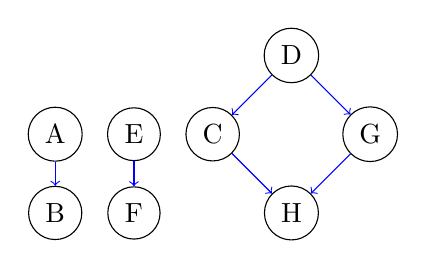
\begin{tikzpicture}
		\mynode[A]{0}{1}
		\mynode[B]{0}{0}
		\mynode[E]{1}{1}
		\mynode[F]{1}{0}
		\mynode[C]{2}{1}
		\mynode[D]{3}{2}
		\mynode[G]{4}{1}
		\mynode[H]{3}{0}
		%	\node [draw] (A) at (0, 0) {A};
		%	\node [draw] (B) at (3, 0) {B};
		%	\node [draw] (C) at (3, 3) {C};
		\relation{A}{B}
		\relation{E}{F}
		\relation{D}{G}
		\relation{D}{C}
		\relation{G}{H}
		\relation{C}{H}
		\end{tikzpicture}
		\caption{Bayesian Network}
		\label{fig:bn1}
	\end{figure}
	
	\subsection{Is the answer above unique?}
	\textbf{No}. As mentioned above H has to be the child of C and G, and D has to be their parents. However, A can be the parent of B, or B can be the parent of A. Same goes for E and F. Thus, there are $ 2^2 $ combinations, which add up to \textbf{4 possible BN that will hold the statements}.
	
	\section{}
	\begin{figure}
		\centering
		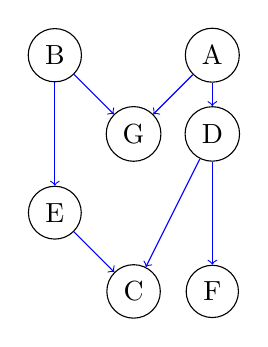
\begin{tikzpicture}
		\mynode[A]{3}{3}
		\mynode[B]{1}{3}
		\mynode[E]{1}{1}
		\mynode[F]{3}{0}
		\mynode[C]{2}{0}
		\mynode[D]{3}{2}
		\mynode[G]{2}{2}

		\relation{A}{D}
		\relation{A}{G}
		\relation{B}{G}
		\relation{B}{E}
		\relation{D}{C}
		\relation{E}{C}
		\relation{D}{F}
		\end{tikzpicture}
		\caption{Network tree}
		\label{fig:bn2}
	\end{figure}
	\subsection{Is this network a poly-tree?}
	\subsection{Is this network (directed-path) singly connected?}
	\subsection{Determine the truth of the following independence statements (using d-separation)}
	\begin{enumerate}		
		\item \begin{verbatim} I({D}, {E} | {    }) - False \end{verbatim}
		Since A is not in evidence, D and G are dependent. Sine B is not in evidence, G and E are dependent. Thus, D and E are dependent.
		\item \begin{verbatim} I({D}, {E} | {  A }) - True \end{verbatim}
		Since A is in evidence, D and G are independent. Since C is not in evidence, there is no path between D and E, therefore they are dependent.
		\item \begin{verbatim} I({D}, {E} | {A, C}) - False \end{verbatim}
		Since C is in evidence, E and D are dependent. 
		\item \begin{verbatim} I({B}, {F} | {  G }) - True \end{verbatim}
		Since G is not in evidence, B and A are independent. Since C is not in evidence, E and D are independent. Therefore, there is no path between B and F, so they are independent.
		\item \begin{verbatim} I({B}, {F} | {  D }) - True \end{verbatim}
		Same as before.
		\item \begin{verbatim} I({B}, {F} | {A, C}) - False \end{verbatim}
		Since C is in evidence, there is a path between B and F so they are dependent.

	\end{enumerate}

	\subsection{Find $P(E=true, A=True | B=true)$}
	\begin{verbatim}
	P(A=true) = 0.2, P(B=true)= 0.3
	P(G=true|A=true,B=true) = 0.9, P(G=true|A=false,B=true) = 0.2
	P(G=true|A=true,B=false) = 0.5, P(G=true|A=false,B=false) = 0.1
	P(E=true|B=true) = 0.8, P(E=true|B=false) = 0.1
	P(C=true|D=true, E=true) = 0
	\end{verbatim}
	
	Since G and C are not in evidence and B is in evidence, we can safely say that A and E are statistically independent. Moreover, A and B are also independent since G and C are not in evidence. Hence
	
	$ P(E, A | B) =P(E|B)*P(A|B)=P(E|B)*P(A)=0.8 * 0.2 = 0.16 $
	
	\section{}
	
	\section{}
	Im general, the utility value for a car is
	\begin{equation}\label{eq:utility}
	U[car] = -(PurchasePrice - SellingPrice +\sum_{year=1}^{3}\gamma^{year}*Kilometer/Year*PriceOfGas/Kilometeru)
	\end{equation}
	At first, the discount factor, $ \gamma $ is 1.
	\subsection{what is your optimal decision?}
	The mean expected price of gasoline (COG) is,
	$$ COG = (0.5 * 1.5 + 0.5 * 3)[MU/liter] = 2.25[MU/liter] $$
	Therefore, the utility, for H and G for the next 3 year of expected 150,000[km] and estimated retail values of the cars are,
	$$ U[H] = -(40,000 [MU] - 20,000[MU] + 4/100[liter/km] * 150,000[km] * 2.25[MU/liter]) = -33.5[KMU] $$
	$$ U[G] = -(25,000 [MU] - 12,500[MU] + 8/100[liter/km] * 150,000[km] * 2.25[MU/liter]) = -39.5[KMU] $$
	Therefore, it would be wise to buy the hybrid car due to higher utility value.
	\subsection{what is your optimal policy based on joining the rioting}
	Based on joining the riot, there is a greater chance in canceling the tax, i.e., now the COG is
	$$ COG = (0.6 * 1.5 + 0.4 * 3)[MU/liter] = 2.1[MU/liter] $$
	In addition, there is a $ 1\% $ chance that riot will have a backfiring cause of 50KMU there fore the utility for buying the H and G when joining the riot is,
		$$ U[H,R] = -(40,000 [MU] - 20,000[MU] + 4/100[liter/km] * 150,000[km] * 2.1[MU/liter] + 50KMU * 0.01) = -33.1[KMU] $$
	$$ U[G,R] = -(25,000 [MU] - 12,500[MU] + 8/100[liter/km] * 150,000[km] * 2.1[MU/liter] + 50KMU * 0.01) = -38.2[KMU] $$
	Therefore, it would be wise to buy the hybrid car and join the riot.
	\subsection{maximum amount you should be willing to pay Picard for this information?}
	Assuming that the riot will have a positive effect on the taxation, the utility for both vehicles will be,
	$$ U[H] = -(40,000 [MU] - 20,000[MU] + 4/100[liter/km] * 150,000[km] * 1.5[MU/liter]) = -29.0[KMU] $$
	$$ U[G] = -(25,000 [MU] - 12,500[MU] + 8/100[liter/km] * 150,000[km] * 1.5[MU/liter]) = -30.5[KMU] $$	
	Therefore, in any scenario it would be wisest to choose to buy a Hybrid, therefore, information has no value if we end up with the same decision. 

	This can also be seen directly from calculation,
	\begin{equation}\label{key}
	\begin{split}{cc}
	VPI & = (TaxRaise * 0.5 + NoTaxRaise * 0.5) - ExpectedValueWithout\\ & = (-29*0.5 + -38 * 0.5) - (-33.5)=0
	\end{split}
	\end{equation}
	
	\subsection{Adding discount}
	For $ \gamma = 0.1 $ using \eqref{eq:utility} will yield
	\subsubsection{what is your optimal decision?}
	$$ U[H] = -(40,000 - 20,000 + 4/100 * 50,000 * 2.25 * (1 + 0.1 + 0.01)) = −24,995$$
	$$ U[G] = -(25,000 - 12,500 + 8/100 * 50,000 * 2.25 * (1 + 0.1 + 0.01)) = −22,490$$
	Best choice now is Gasoline car.
	\subsubsection{what is your optimal policy based on joining the rioting}
	$$ U[H] = -(40,000 - 20,000 + 4/100 * 50,000 * 2.1 * (1 + 0.1 + 0.01)+ 50,000 * 0.01) = −25,162$$
	$$ U[G] = -(25,000 - 12,500 + 8/100 * 50,000 * 2.1 * (1 + 0.1 + 0.01)+ 50,000 * 0.01) = −22,324$$	
	Best choice now is Gasoline car.	
	\subsubsection{maximum amount you should be willing to pay Picard for this information?}
	Assuming that the riot will have a positive effect on the taxation, the utility for both vehicles will be,
	$$ U[H] = -(40,000 - 20,000 + 4/100 * 50,000 * 1.5 * (1 + 0.1 + 0.01)) = −23,330$$
	$$ U[G] = -(25,000 - 12,500 + 8/100 * 50,000 * 1.5 * (1 + 0.1 + 0.01)) = −19,160$$		
	Once again, information has no impact on decision, therefore no value for information.
	
	\section{}
	\begin{figure}[H]
		\centering
		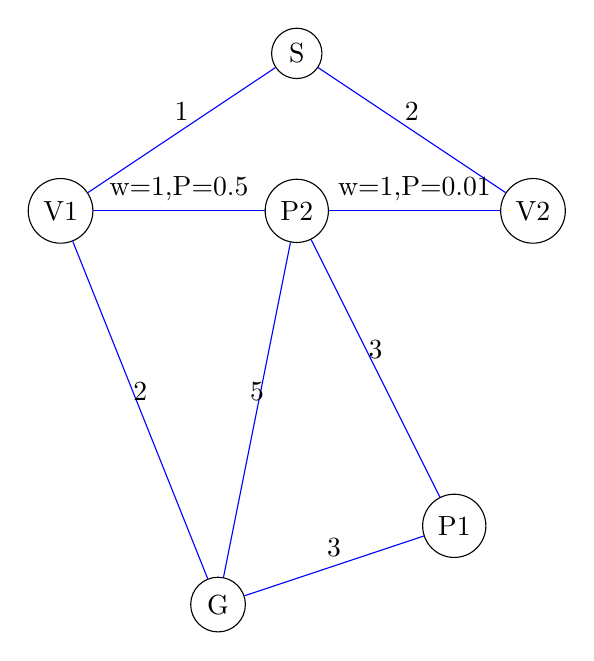
\begin{tikzpicture}
		\mynode[S]{3}{7}
		\mynode[V1]{0}{5}
		\mynode[P1]{5}{1}
		\mynode[G]{2}{0}
		\mynode[P2]{3}{5}
		\mynode[V2]{6}{5}
		
		\wrelation[1]{S}{V1}
		\wrelation[w=1,P=0.5]{V1}{P2}
		\wrelation[2]{V1}{G}
		\wrelation[2]{S}{V2}
		\wrelation[w=1,P=0.01]{V2}{P2}
		\wrelation[3]{P1}{G}
		\wrelation[3]{P1}{P2}
		\wrelation[5]{G}{P2}		
		\end{tikzpicture}
		\caption{Hurricane graph.}
		\label{fig:hurricane}
	\end{figure}

	\subsection{Formalize the above problem as a MDP}
	\subsubsection{States}
	The states should hold the entire information of the realm. Therefore, a state would be a tuple with the following structure:
	\begin{equation}\label{eq:state}
	 state = (l, T, PIV, R, P1, P2, B(V2, P2), B(V1, P2)) 
	\end{equation}
	where, $ l $ is the current vertex the agent is at, $ T $ is the remaining time, $ PIV $ is the amount of people in the vehicle, $ R $ is the amount of people rescued, $ P_i $ is a Boolean representing the presence of people at the vertex, and $ B(x, y) $ is a triple valued variable stating if the edge between x and y is blocked / unblocked or unknown.
	
	\subsubsection{Reward}
	The only reward of interest in this scenario is the amount of people saved. Therefore, each person that was rescued will provide 1 reward, and rewards are given when the agent reaches shelter (G vertex in this example). All other transitions are 0 reward. 
	\begin{equation}\label{key}
	Reward = \left\{ \begin{array}{c}
	PIV \quad if(l==shelter) \\
	0 \quad otherwise
	\end{array} \right.
	\end{equation}
	
	\subsubsection{transition}
	Moving from state to state reduces the time, changes the amount of people saved or picked up and reviles if edges  are blocked or not. When planning a route, the probability of blockages are taken into account. For example, the utility for the transition from state $ S(x, ...) $ to $ S(y, ...)^\prime` $
	\begin{equation}\label{eq:transition}
	U[S^\prime] = U[S] * (1 -P(B(x, y))+Reward
	\end{equation} 
	
	\subsection{Find the optimal policy}
	From S there are two options: going to V1 and going to V2. If the agent will go to V2 and the edge (V2, P2) is blocked, the agent will have to go back to S and there will not be enough time to save people. However, if  the edge is unblocked, the agent will be able to save all three people (i.e. $ S\rightarrow V2\rightarrow P2\rightarrow P1\rightarrow G $).
	Since the probability of blockage is $ 1\% $ the utility of going to V2 is:
	\begin{equation}\label{uv2}
	U[S\rightarrow V2]  = 3 * 99\% + 0 * 1\% = 2.97
	\end{equation}
	
	However, if the agent will go to V1, there is a $ 50\% $ chance that the edge (V1, P2) is blocked. If it is blocked the agent would still save P1. If it is unblocked, the agent will save all 3 people. Therefore, the utility for going to V1 will be,
	\begin{equation}\label{key}
	U[S\rightarrow V1] = 3 * 50\% + 1 * 50\% = 2
	\end{equation}
	
	Therefore, the best policy would be to go to V2 as there is higher chance to save all 3 people.
	
	
	\section{}
	
	\section{}
	\subsection{Can this be done without hidden units?}
	\textbf{No.} It is impossible with no hidden layers to predict a non-linear function such as modulu. However, for this simple example, a single hidden layer will suffice as shown in the following subsection.
	
	\subsection{Show a network using threshold elements that performs the required computation}
	We will use a neural network with 1 hidden layers that is composed of 6 neurons. This means for the input layer (6 neurons), the hidden layer will have 36 weights (6 x 6 matrix - M1) and 6 bias weights that are summed and enter a $ tanh $ activation function. 
	
	The output, a 6x1 vector $ X1 $ is then bitwise multiplied by 6 weights (one for each neuron) summed and are added with the bias $ b2 $. The output is passed through a sigmoid activation function and the result is rounded to decide if the result is '0' or '1'.
	
	The complete code in Keras that generates the dataset and labels, trains, and provides the weights can be found, along with this report, in the git repository at \url{https://github.com/odedyec/IntroToAI/blob/master/assignment6/q7.py}. This network, after 500 epochs completely learns the model and every input is correctly classified.
	\begin{equation}\label{eq:m1}
	M1 = \left[ \begin{array}{cccccc}
		-2.6035163 & 1.0730004 & 0.73517716 &  0.7892835 & 2.0436563 & -3.0340612 \\
		-2.8252845 & 1.1691521 & 1.3764652 & 1.5624126 & -3.209769 &	-2.571492  \\
		-2.5988533 & 1.1376183 & 0.9316116 & 0.563356  & 2.0437527 & -3.031866  \\
		-2.5722306 & 1.2495581 & 0.7956654 & 0.7881598 & 2.0363252 &	-3.0355027 \\
		-2.603346  & 1.1103705 & 0.60637933 & 0.61684054 & 2.0353322 & -3.025518 \\
		-2.5890596 & 1.0401373 & 0.26387808 & 1.0831383 & 2.0149522 &  -3.0376844 \\
	\end{array} \right]
	\end{equation}
	\begin{equation}\label{eq:b1}
	b1 = \left[8.979317  , -5.988329  ,  0.26482144, -0.250453  , -1.1340998 ,
	6.665368 \right]^T
	\end{equation}
	\begin{equation}\label{eq:m2}
	M2 = \left[\begin{array}{c}
	6.996323 \\
	  4.3360047\\
	 -0.807298\\
	 -0.6610357\\
	 -1.4745305\\
	-10.0931015
	\end{array}\right]
	\end{equation}
	\begin{equation}\label{eq:b2}
	b2 = -2.8664327
	\end{equation}
	\begin{equation}\label{eq:l1}
	X1 = tanh(M1 \times X + b1)
	\end{equation}
	\begin{equation}\label{eq:l2}
	\hat{y} = round(sigmoid(M2 \times X1) + b2)
	\end{equation}
\end{document}

